\documentclass[conference,10pt,letterpaper]{IEEEtran}
\IEEEoverridecommandlockouts
% The preceding line is only needed to identify funding in the first footnote. If that is unneeded, please comment it out.
\usepackage{cite}
\usepackage{amsmath,amssymb,amsfonts}
\usepackage{algorithmic}
\usepackage{graphicx}
\usepackage{textcomp}
\usepackage{xcolor}
\usepackage{fancyhdr}
\usepackage[hidelinks]{hyperref} % Include this package to use hyperlinks
\usepackage{stfloats}
\usepackage{tabularx}
\usepackage{ulem}

% Set single spacing
\linespread{1}

% Times New Roman font (if required, uncomment the next line)
\usepackage{times}

\def\BibTeX{{\rm B\kern-.05em{\sc i\kern-.025em b}\kern-.08em
		T\kern-.1667em\lower.7ex\hbox{E}\kern-.125emX}}
	
%\setlength{\parindent}{0pt}	

\begin{document}
	
	\title{Wattson: An Innovative IELTS Speaking Assistant Android Application}
	
	\author{
		\IEEEauthorblockN{Kaijie Lai }
		\IEEEauthorblockA{2034675\\
			\href{mailto:Kaijie.Lai20@student.xjtlu.edu.cn}{Kaijie.Lai20@student.xjtlu.edu.cn} }
	}
	\maketitle
	
	%header
	\pagestyle{fancy} % This sets the fancy style for all pages
	\fancyhead[LO,L]{CAN 301}
	\fancyhead[CO,C]{Mobile Computing}
	\fancyhead[RO,R]{\today}
	\fancyfoot[LO,L]{}
	\fancyfoot[CO,C]{\thepage}
	\fancyfoot[RO,R]{}
	\renewcommand{\headrulewidth}{0.4pt}
	\renewcommand{\footrulewidth}{0.4pt}
	
	\section{Introduction}
	\begin{figure*}[b]
		\centering
		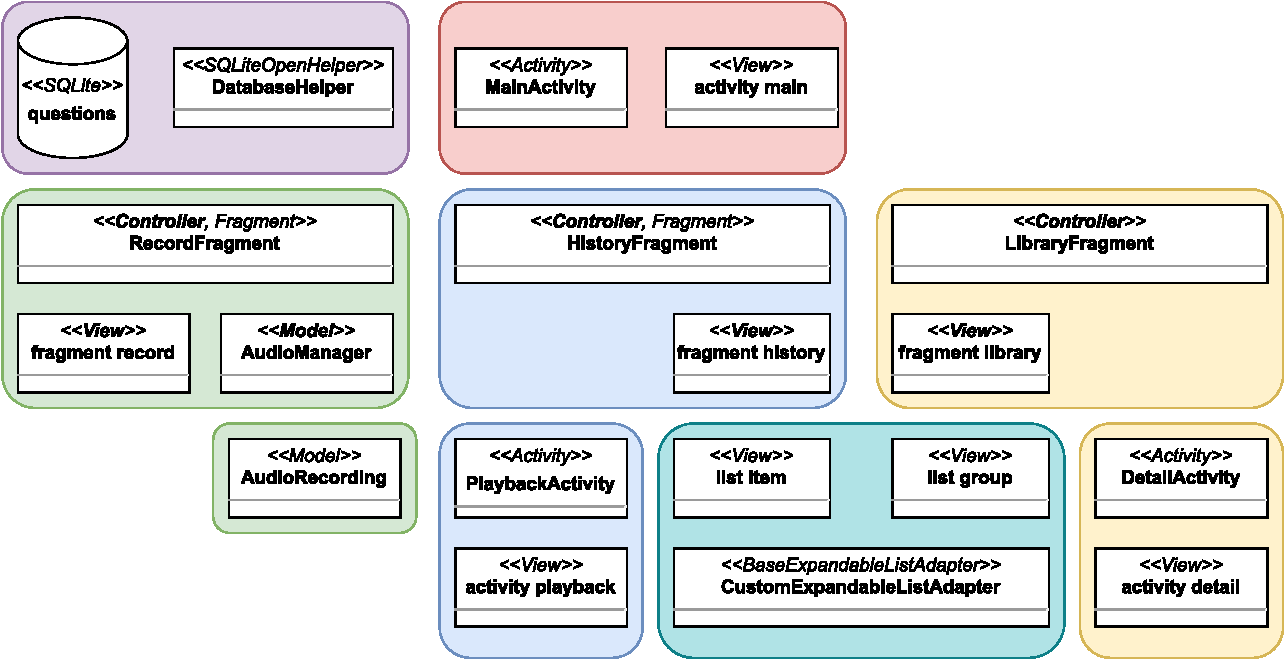
\includegraphics[width=6.2in]{src/all-classes.pdf}
		\caption{MVC Architecture of Project}
		\label{fig:all_classes}
	\end{figure*}
	
	This report presents development and evaluation of "Wattson", an innovative IELTS Speaking Assistant Android application designed to aid students in IELTS speaking practice. The report details the app design, including its user interface and functional features, followed by an evaluation of its effectiveness in aiding IELTS speaking preparation. 
	
	\subsection{Motivation}
	As a student at Xi'an Jiaotong-Liverpool University, where the majority of students aspire to pursue postgraduate studies abroad, proficiency in the IELTS exam is a common requirement. Among the various sections of the IELTS, the speaking part often poses the greatest challenge for Chinese students.
	
	In my personal experience preparing for the IELTS, I realized that achieving a high score necessitates repetitive practice and training. Recording and reviewing one's own spoken responses is a straightforward and effective method for improvement. However, existing software for oral training on the market are either focused on isolated practice sessions (such as casual conversation practice with a peer) or, like voice assistant apps (e.g. \href{https://callannie.ai/}{Call Annie}), lack targeted training features.
	
	Typically, practice involves the cumbersome process of operating a recorder while simultaneously opening a file of speaking prompts on a computer, selecting a question, and then starting the recording on the phone. Recognizing the inefficiency of this method led me to conceptualize a software solution that combines these two elements. This app aims to streamline the IELTS speaking practice by integrating a database of questions with an easy-to-use recording feature, allowing users to focus on enhancing their speaking skills without the hassle of juggling multiple devices or applications.
	
	\subsection{Contribution}
	Generally speaking, I authored most of the code for this project. In this individual report, I will specifically discuss the Record Part and Navigation Feature, highlighting my contributions to these areas. The entire project is designed based on the Model-View-Controller (MVC) architecture in Figure \ref{fig:all_classes}. Additionally, I will detail the operational logic of the application, as well as the testing environment, and provide a user guide for understanding and interacting effectively.
	
	\newpage
	\section{App Design}
	
	In this section, we delve into the intricacies of two primary features of our application: the Record feature and the Bottom Navigation. These features are dissected from multiple perspectives to provide a comprehensive understanding of their design and functionality.
	
	\subsection{Record Feature}
	The Record feature is a crucial component of the app, and its design is considered from the following aspects:
	\begin{enumerate}
		\item \textbf{User Interface (UI)}: 
		The primary components of the View for the Record feature are defined in the \texttt{res/layout/fragment\_record.xml}. The corresponding class diagram illustrates the object structure in Figure \ref{fig:record_part}. Initially, the UI layout is as shown in the schematic Figure \ref{fig:record_layout}. Interaction and visibility of different UI elements, such as buttons, are controlled in \texttt{RecordFragment} by modifying their visibility attributes (visible, invisible, or gone). The View utilizes components like \texttt{TextView}, \texttt{View}, \texttt{SeekBar}, and \texttt{ImageButton}, while the ViewGroup includes \texttt{FrameLayout}, \texttt{LinearLayout}, and \texttt{GridLayout}. The app's theme, set in \texttt{values/themes/themes.xml}, employs a \texttt{NoActionBar} style for a clean interface without a primary bar. Colors used throughout the application are defined in \texttt{values/colors.xml}, and all fundamental strings are set in \texttt{values/strings.xml}.
		\begin{figure}[htbp]
			\centerline{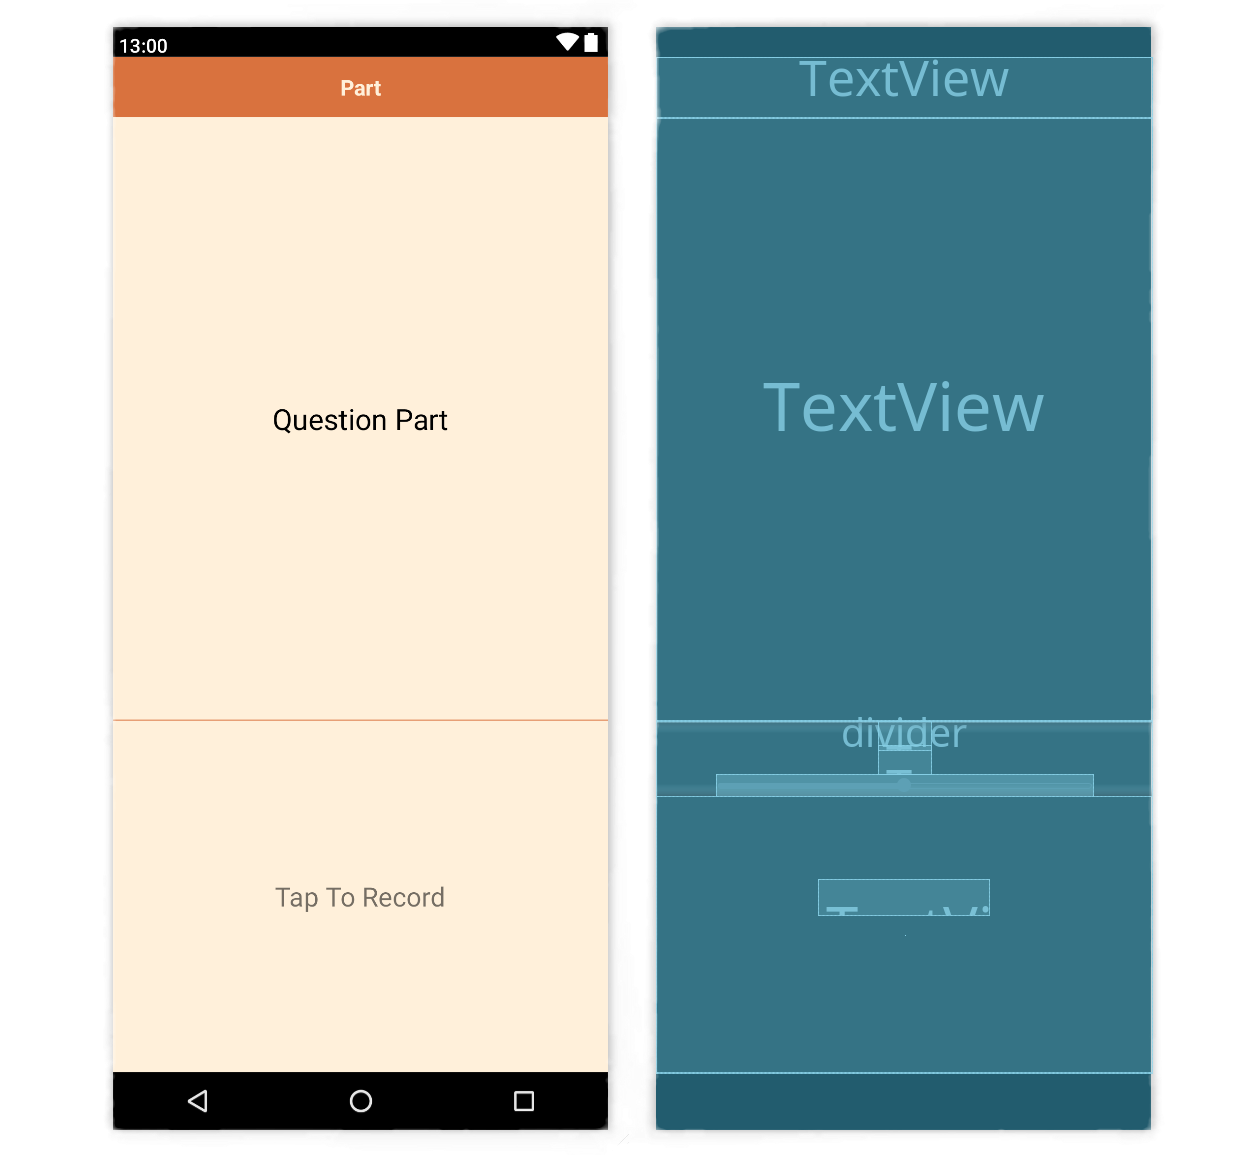
\includegraphics[width=\columnwidth]{src/record layout remove.png}}
			\caption{Layout View of Record Fragment}
			\label{fig:record_layout}
		\end{figure}
		
		\item \textbf{User Experience (UX)}: 
		Upon opening the app, users are automatically directed to the Record Part (as shown in the attached Figure \ref{fig:record_part}). At the top of the page, users see a question from the database along with its corresponding Part. Following the prompt \texttt{Tap to record} begins the recording process. A subsequent tap changes the prompt to \texttt{Tap to pause}, allowing users to pause the recording. Options then include \texttt{Tap to resume} or \texttt{Long press to finish}. After recording, users can see their recording with options to play it back by pressing the play button and navigate through the recording using the progress bar. The \texttt{Next} button allows users to proceed to the next question, saving the current recording. If unsatisfied, the \texttt{Delete} option is available to remove the recording, accompanied by a system prompt for confirmation and a toast message \texttt{Recording deleted successfully} upon deletion. This workflow constitutes the entire user experience of the Record functionality in the flowchart Figure \ref{fig:flowhart}.
		\begin{figure}[htbp]
			\centerline{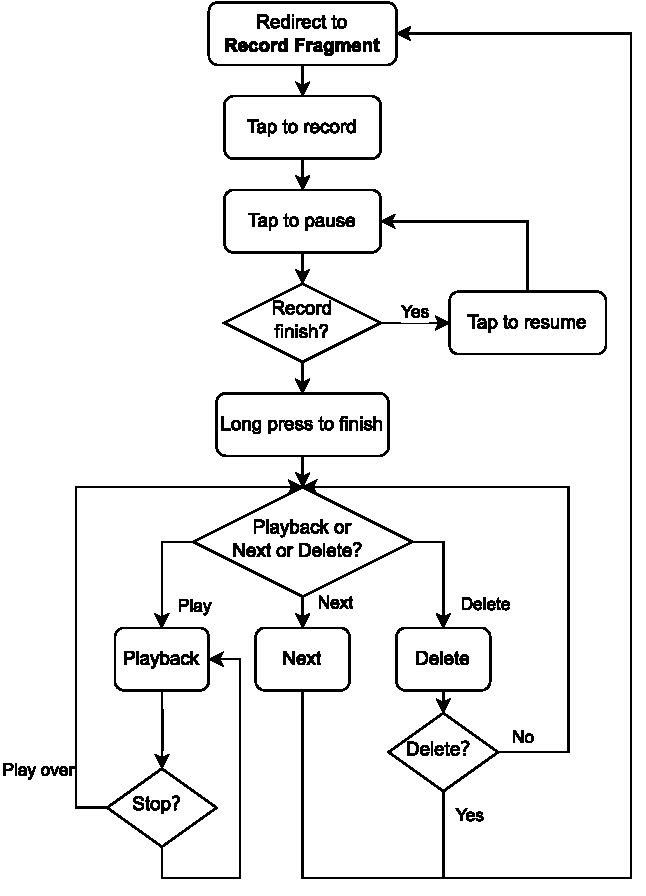
\includegraphics[width=3.1in]{src/flowchart.pdf}}
			\caption{Flowchart of Record Instruction}
			\label{fig:flowhart}
		\end{figure}
		
		\begin{figure*}
			\centering
			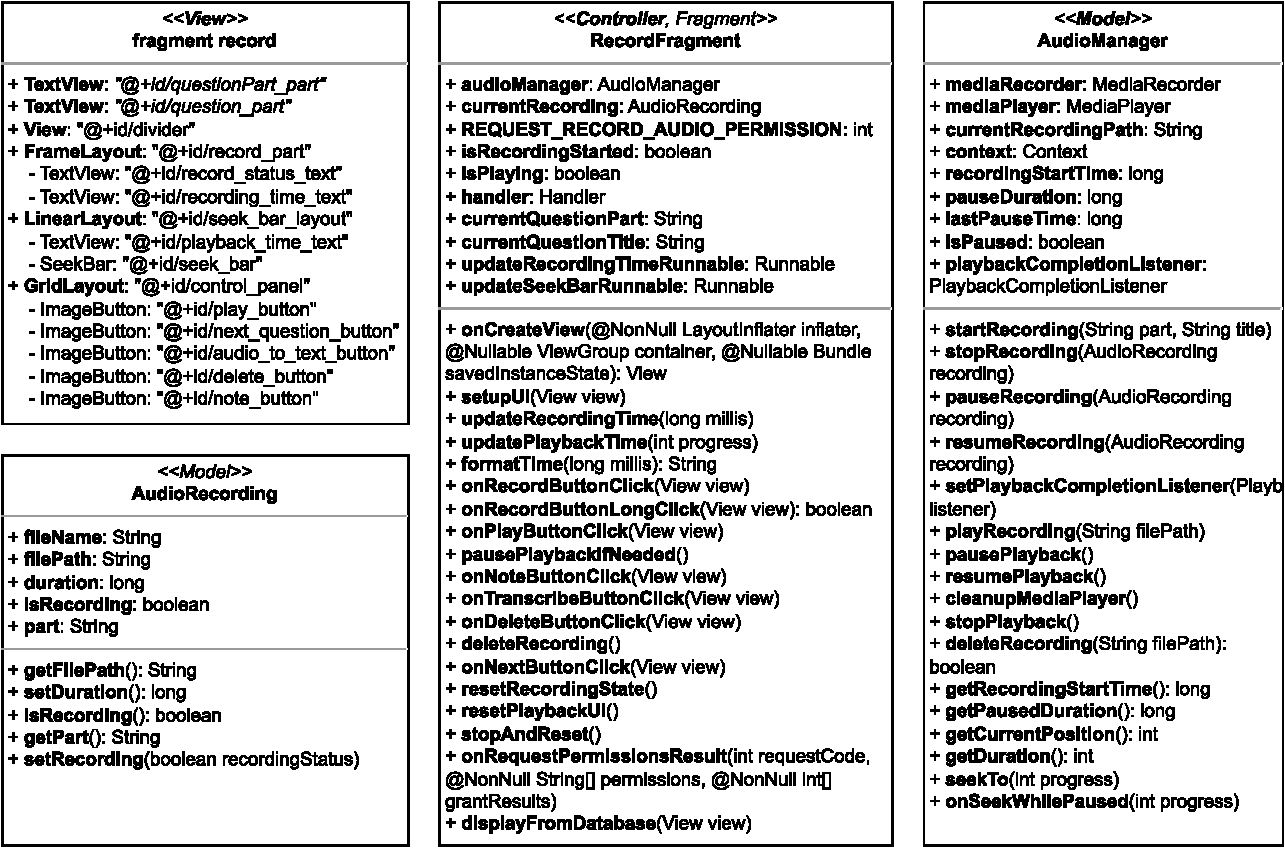
\includegraphics[width=6.2in]{src/record part.pdf}
			\caption{Classes Diagram of Record Part}
			\label{fig:record_part}
		\end{figure*}
		
		\item \textbf{Permissions and Data Management}: 
		The \texttt{RecordFragment} class manages permissions and data intricately. It checks for audio recording permissions using the \texttt{ContextCompat.checkSelfPermission} method and requests them if not already granted. This ensures that the app adheres to Android's security norms. Additionally, the class interacts with the \texttt{DatabaseHelper} like in Figure \ref{fig:datahelper} to retrieve and display questions from the database. This involves fetching random questions and their corresponding details, demonstrating the app's ability to manage and utilize data effectively. The management of audio files, such as creation, playback, and deletion, is handled through the \texttt{AudioManager} class, showcasing a well-structured approach to data handling and storage.
		\begin{figure}[htbp]
			\centerline{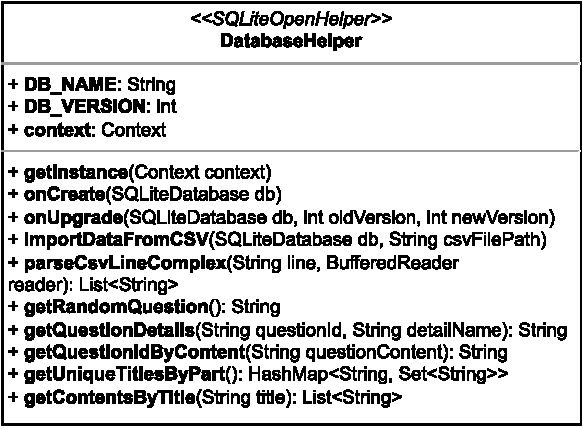
\includegraphics[width=3in]{src/datahelper.pdf}}
			\caption{Class of Datahelper}
			\label{fig:datahelper}
		\end{figure}
		
		\item \textbf{Error Handling and User Feedback}: 
		The code demonstrates careful consideration of error handling and user feedback. For instance, if the \texttt{Question TextView} or \texttt{Part TextView} is null, the app logs an error message, indicating a fail-safe approach to null pointer exceptions. During operations like deleting a recording, the app provides user feedback through \texttt{Toast} messages, such as "Recording deleted successfully" or "Failed to delete recording", enhancing the user experience. The use of confirmation dialogs before deleting recordings is another example of thoughtful user interaction design. Moreover, the app logs various actions and errors, such as in \texttt{displayFromDatabase} and \texttt{onDeleteButtonClick} methods, which aids in troubleshooting and ensures a smooth user experience.
		
		\item \textbf{Functionality Implementation}: 
		The implementation of the Record Fragment's functionality is illustrated in the sequence diagram in Figure \ref{fig:record_sequence} shown below. This diagram clearly depicts the flow of operations within the Record Fragment, providing a visual representation of the interactions and processes involved. The sequence diagram aids in understanding the sequential steps and the logical flow of the recording feature, from initiating a recording to handling playback and user interactions.
		
		\begin{figure}[htbp]
			\centerline{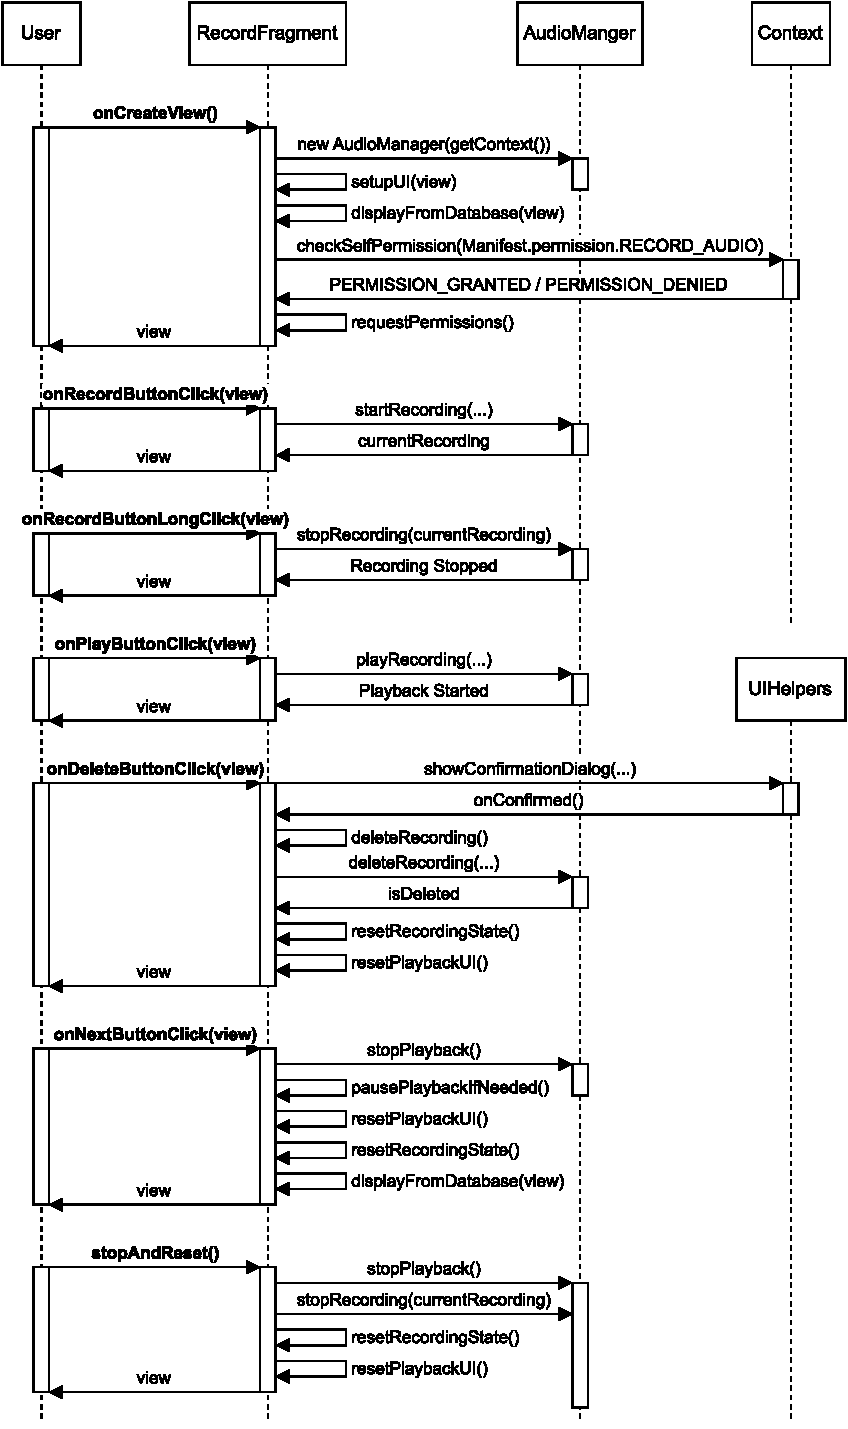
\includegraphics[width=\columnwidth]{src/record-sequence.pdf}}
			\caption{Sequence Diagram of RecordFragment}
			\label{fig:record_sequence}
		\end{figure}

		\item \textbf{Performance Considerations}: 
		The performance of the application during various stages of interaction in the Record Part is a critical aspect of the user experience. The following Table \ref{tab:performance} presents a detailed analysis of the performance metrics associated with different events. These metrics include the duration of each event in milliseconds, CPU usage percentage, and memory usage in megabytes. The data provides valuable insights into the application's responsiveness and efficiency in resource utilization during key interactions such as starting and pausing recording, resuming recording, finishing recording, playback, and other functionalities. This analysis is instrumental in identifying potential areas for optimization to enhance the performance of the app.
		\begin{table*}[!b]
			\centering
			\begin{tabularx}{6.2in}{|X|X|X|X|X|}
				\hline
				\textbf{Event} & \textbf{Stage} & \textbf{\textit{Duration (ms)}} & \textbf{\textit{CPU Usage (\%)}} & \textbf{\textit{Memory Usage (MB)}} \\ \hline
				Touch Event Press & Start Record  & \textit{51.48}  & \textit{1}            & \textit{49.2} \\ \hline
				Touch Event Press & Record Pause  & \textit{71.09}  & \textit{2}            & \textit{49.3} \\ \hline
				Touch Event Press & Resume Record & \textit{91.21}  & \textit{\textless{}1} & \textit{49.2} \\ \hline
				Touch Event Press & Record Finish & \textit{882.02} & \textit{1}            & \textit{49.1} \\ \hline
				Touch Event Press & Playback      & \textit{143.09} & \textit{\textless{}1} & \textit{49.2} \\ \hline
				Touch Event Press & Stop Playback & \textit{147.17} & \textit{\textless{}1} & \textit{49.3} \\ \hline
				Touch Event Press & Next          & \textit{142.03} & \textit{2}            & \textit{49.7} \\ \hline
				Touch Event Press & Delete        & \textit{103.32} & \textit{7}            & \textit{50.1} \\ \hline
			\end{tabularx}
			\caption{Performance Metrics for Record Part Progress}
			\label{tab:performance}
		\end{table*}
		
	\end{enumerate}

	\newpage
	\section{Evaluation}
	\subsection{Challenges}
	During the development of our application, several significant challenges were encountered. These include engineering difficulties, user interface concerns, and other issues pertinent to app development. For instance, a major challenge was how to accurately implement the opening and closing of \texttt{RecorderMedia} and \texttt{PlayMedia}. This issue was critical because improper release of resources could lead to severe crashes, affecting both the stability and reliability of the application.
	
	\subsection{Solutions}
	To address these challenges, various solutions were considered. This included the use of \texttt{Log} and \texttt{Toast} messages during development for situational assessment, as well as the establishment of an \texttt{AudioManager} object to specifically manage \texttt{RecorderMedia} and \texttt{PlayMedia}. Additionally, dedicated \texttt{Recording} objects were used for sound management. These measures successfully resolved the issues, enhancing the app’s functionality and user experience.
	
	\subsection{HCI}
	In terms of Human-Computer Interaction, careful consideration was given to the app's usability. For the \texttt{Tap to record} feature, the lower third of the screen was chosen for interaction, as this area is most easily accessible with the thumb, making it convenient for users. This design allows users to start, pause, resume, and stop recording effortlessly, which is highly beneficial for concentrating on their oral practice without the need to constantly look at the phone. After recording, the interface efficiently uses three ImageButtons to execute different functions, making the app more intuitive and user-friendly.
	
	\subsection{Functionality and Integration}
	Regarding the question of whether the features of our app work as intended and their synergy with other features, the Record Part has been successfully implemented and integrates well with the overall functionality of the app. However, due to the solo nature of the development process and academic pressures, including language exams and assignments, two features could not be completed in time. These are the manual note-taking feature and the implementation of voice-to-text conversion using Android's native APIs.
	
	\subsection{Future Enhancements and Reworked Design}
	Given more time and resources, several enhancements and reworks are envisioned for the app. Keeping in mind the lecture on context awareness, the following improvements are proposed:
	\begin{enumerate}
		\item \textbf{Enhanced Context Awareness:} Incorporating more advanced context-aware features, such as adjusting the difficulty level of questions based on the user's proficiency and learning pace, would make the app more responsive to individual needs.
		
		\item \textbf{Interactive Note-Taking Feature:} As previously mentioned, the manual note-taking feature was not completed. With additional time, this feature would be implemented to allow users to jot down notes or key points during their practice sessions, enhancing the learning experience.
		\item \textbf{Voice-to-Text Functionality:} Implementing the voice-to-text feature using Android's APIs would allow users to see a transcription of their spoken responses, aiding in self-assessment and improvement.
		\item \textbf{UI/UX Rework:} Based on user feedback and HCI principles, the user interface and experience could be further refined. This might include simplifying navigation, making the app more intuitive, and enhancing visual appeal to keep users engaged.
	\end{enumerate}
	
	These proposed enhancements and redesigns are aimed at making the app not only more user-friendly but also more effective as a language learning tool, leveraging the potential of technology to provide a personalized and engaging learning experience.
	
	\section{Conclusion}
	In conclusion, I successfully navigated through key issues in engineering and interface design, implementing effective solutions that have significantly improved the app's performance and usability. My focus on human-computer interaction principles has resulted in an intuitive and accessible tool for IELTS speaking practice. Wattson stands as a testament to the effectiveness of thoughtful design and user-centered development in creating applications that are not only functional but also user-friendly. I believe that this app will make a substantial difference in assisting users in their language learning journey.
	
	\newpage
	\appendix
	\section{Appendix}
	\subsection{Project Repository}
	The source code and additional resources for this project are available in the GitHub repository at the following URL:
	
	\uline{\url{https://github.com/jonlai211/Wattson}}
	
	\subsection{Shortcuts}
	\begin{figure}[htbp]
		\centerline{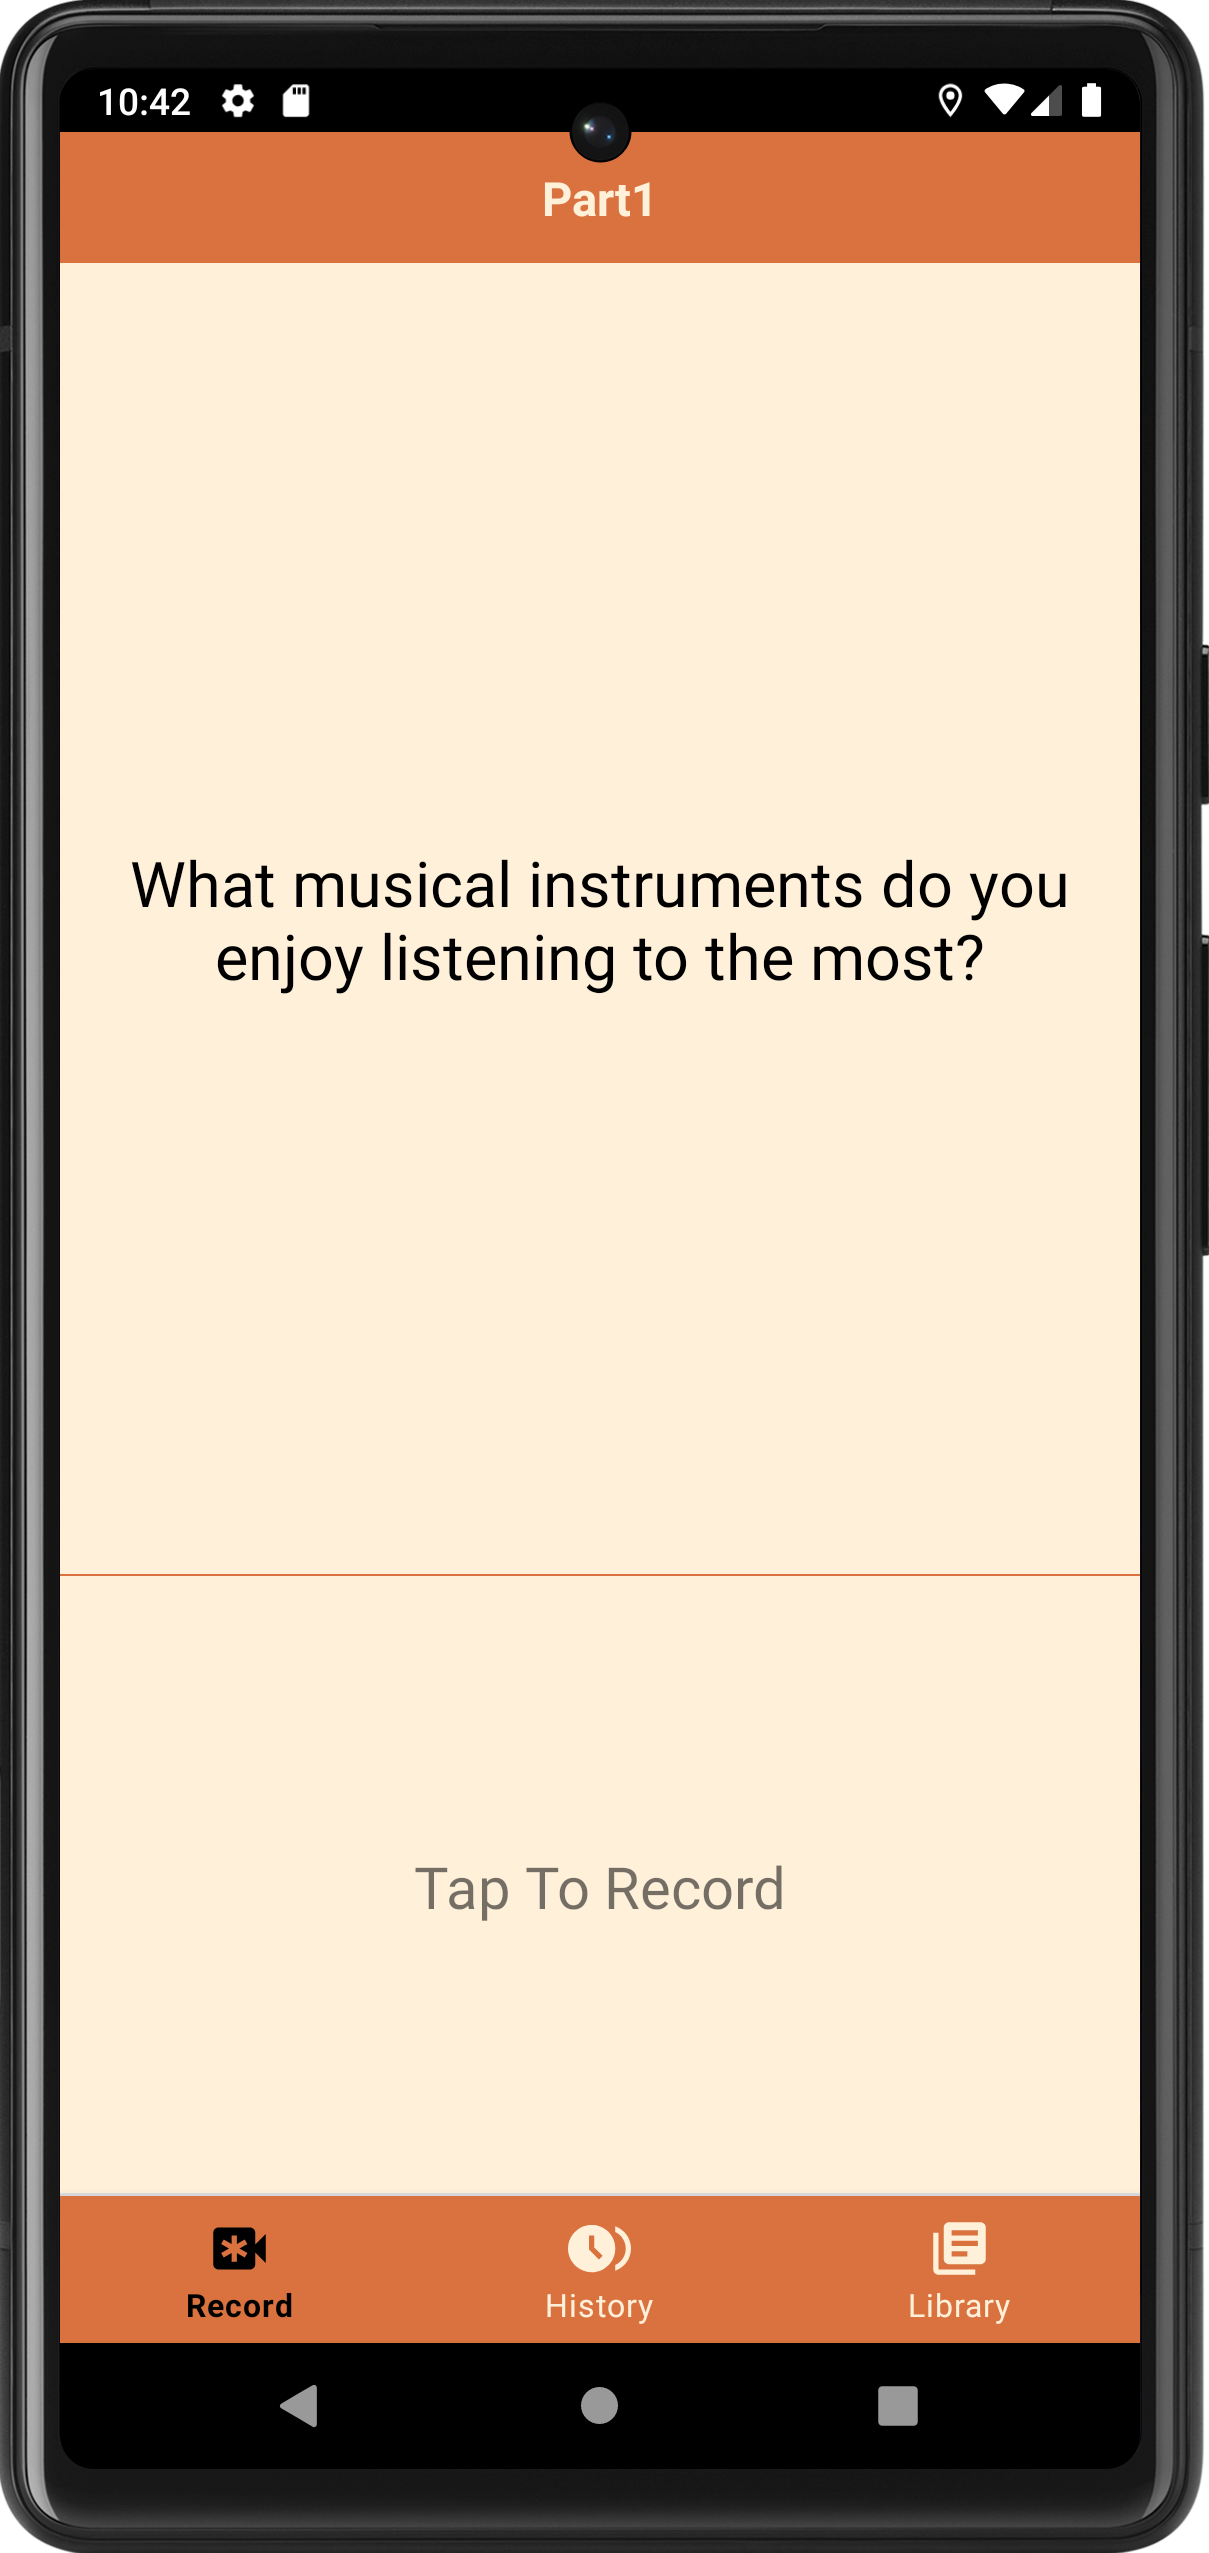
\includegraphics[height=3.5in]{src/record shortcut.png}}
		\caption{Record Shortcut}
		\label{fig:record_shortcut}
	\end{figure}
	
	\begin{figure}[htbp]
		\centerline{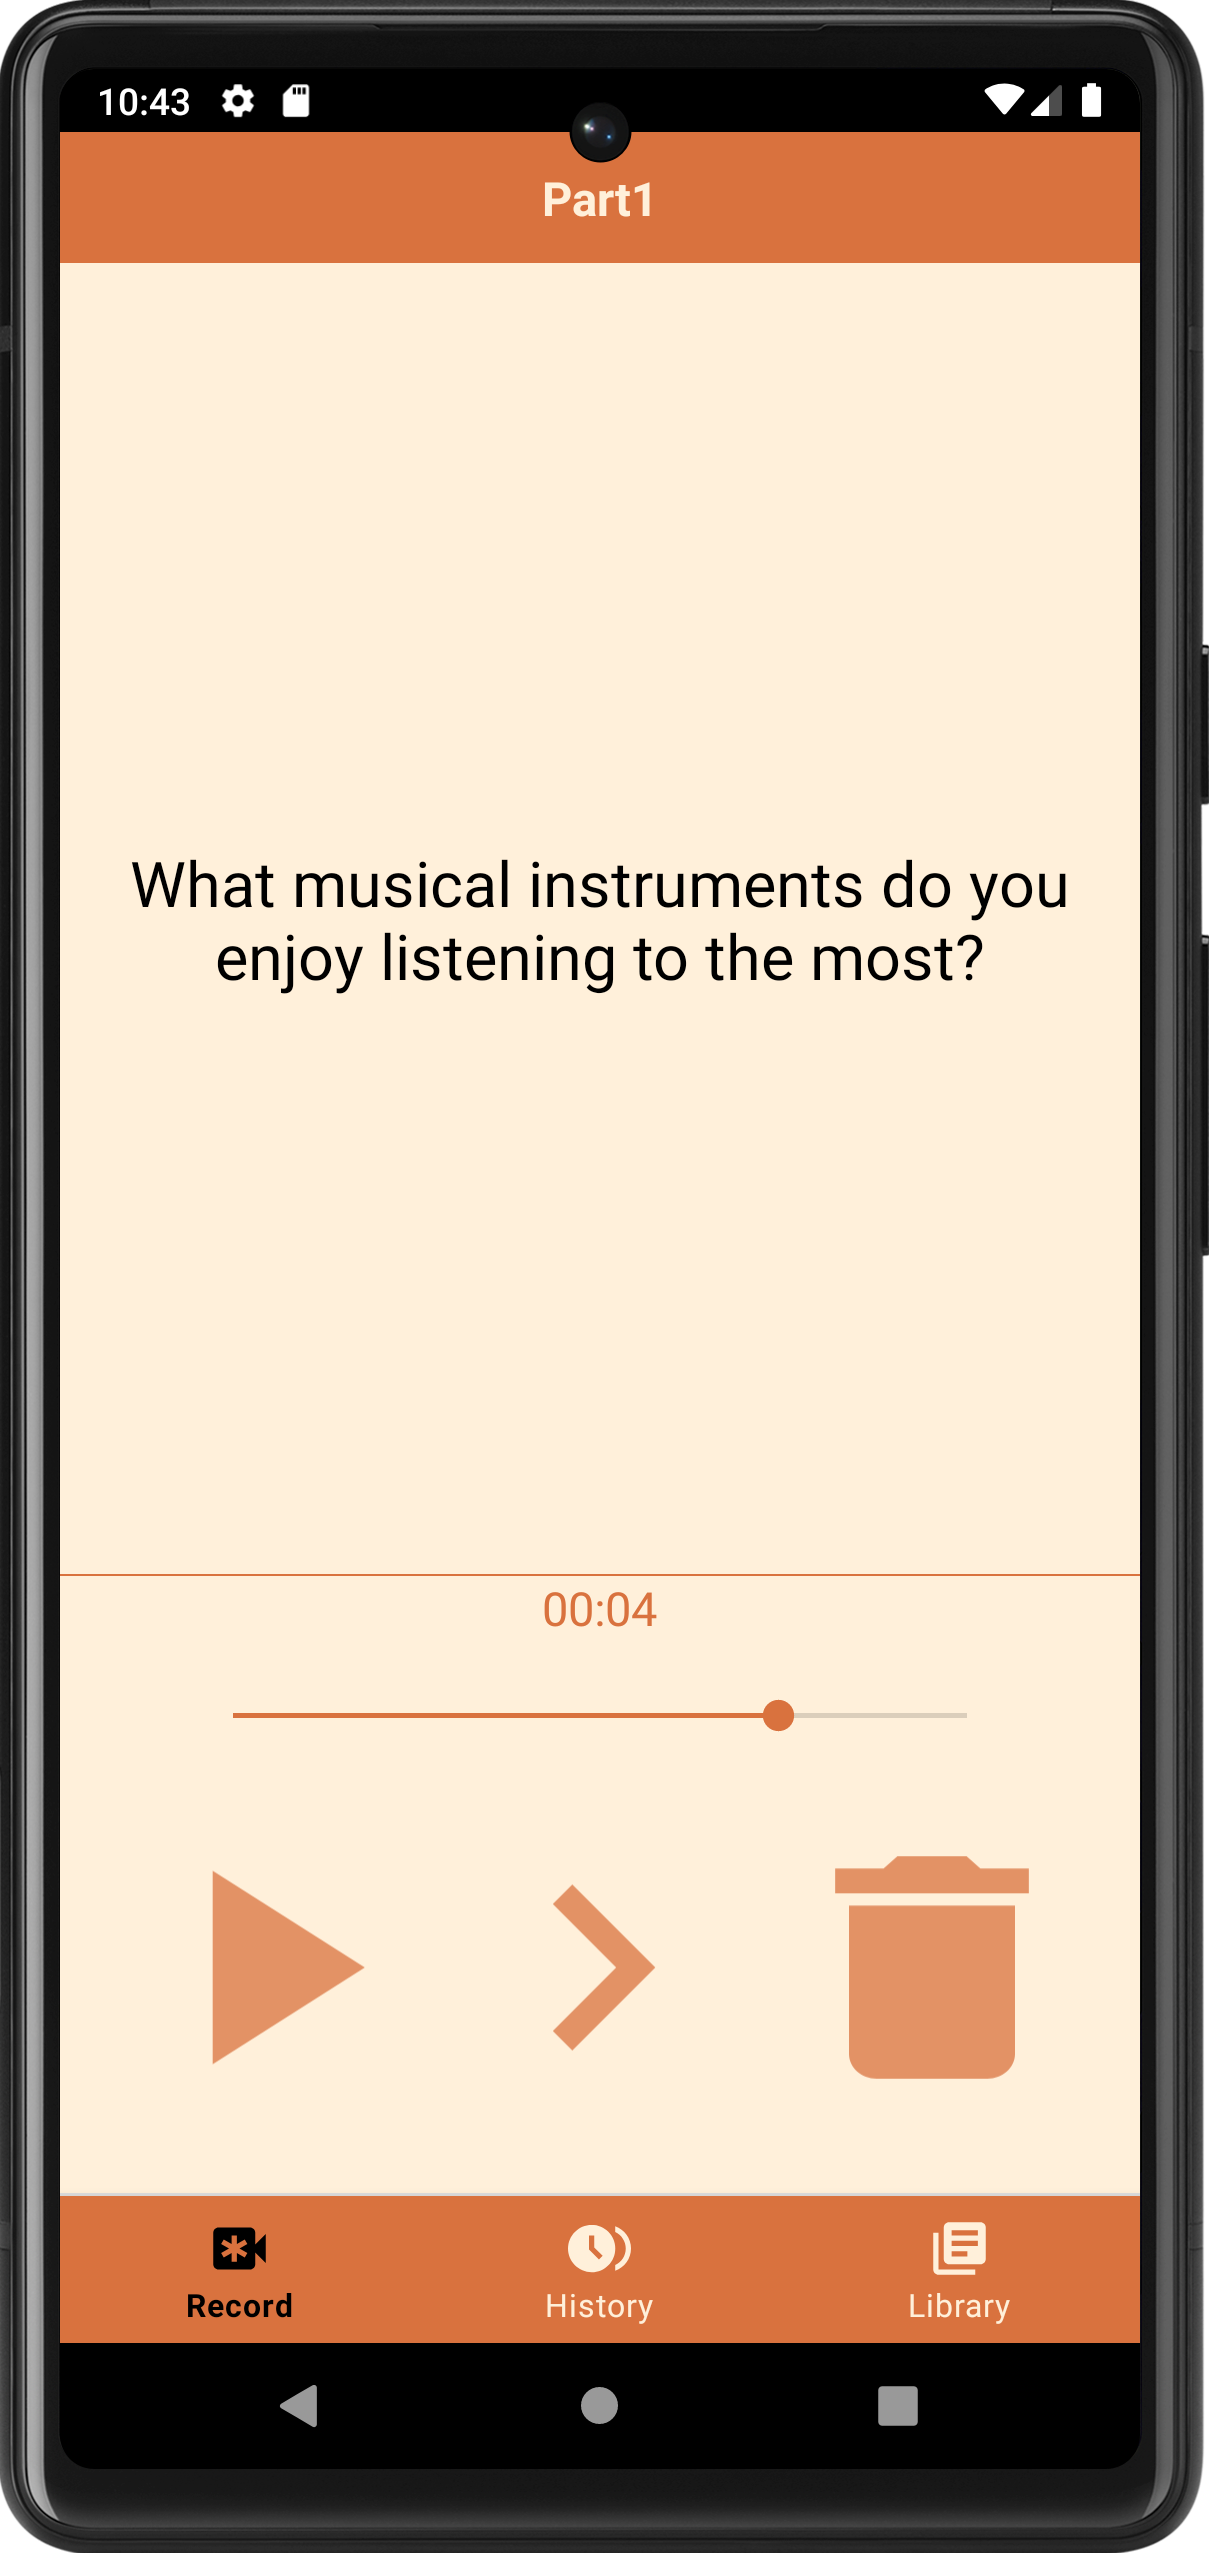
\includegraphics[height=3.5in]{src/control shortcut.png}}
		\caption{Control Shortcut}
		\label{fig:control_shortcut}
	\end{figure}
	
\end{document}
